\documentclass[aspectratio=169]{beamer}

% --- Packages ---
\usepackage[utf8]{inputenc}
\usepackage[T1]{fontenc}
\usepackage{graphicx}
\usepackage{xcolor}
\usepackage{tikz}
\usepackage{listings}
\usepackage{booktabs}
\usepackage{hyperref}

% --- Custom Colors (Premium IoT Theme) ---
\definecolor{IoTDarkBlue}{HTML}{0A192F}
\definecolor{IoTCyan}{HTML}{64FFDA}
\definecolor{IoTGrey}{HTML}{8892B0}
\definecolor{IoTWhite}{HTML}{E6F1FF}

% --- Beamer Theme Customization ---
\setbeamercolor{palette primary}{bg=IoTDarkBlue, fg=IoTCyan}
\setbeamercolor{palette secondary}{bg=IoTDarkBlue, fg=IoTWhite}
\setbeamercolor{palette tertiary}{bg=IoTCyan, fg=IoTDarkBlue}
\setbeamercolor{background canvas}{bg=IoTDarkBlue}
\setbeamercolor{normal text}{fg=IoTWhite}
\setbeamercolor{structure}{fg=IoTCyan}
\setbeamercolor{title}{fg=IoTCyan}
\setbeamercolor{frametitle}{fg=IoTCyan}

\setbeamertemplate{navigation symbols}{}
\setbeamertemplate{footline}[frame number]

% --- Title Page Info ---
\title{IoT Workshop: Building the Connected World}
\subtitle{Session 1: The IoT Ecosystem}
\author{Sanket Salvi}
\institute{NIT Karnataka}
\date{May 2026}

% --- Graphics Path ---
\graphicspath{{../assets/}}

\begin{document}

% --- Title Slide ---
{
\setbeamertemplate{footline}{} 
\begin{frame}
    \titlepage
    \centering
    \begin{tikzpicture}[remember picture,overlay]
        \node[opacity=0.1] at (current page.center) {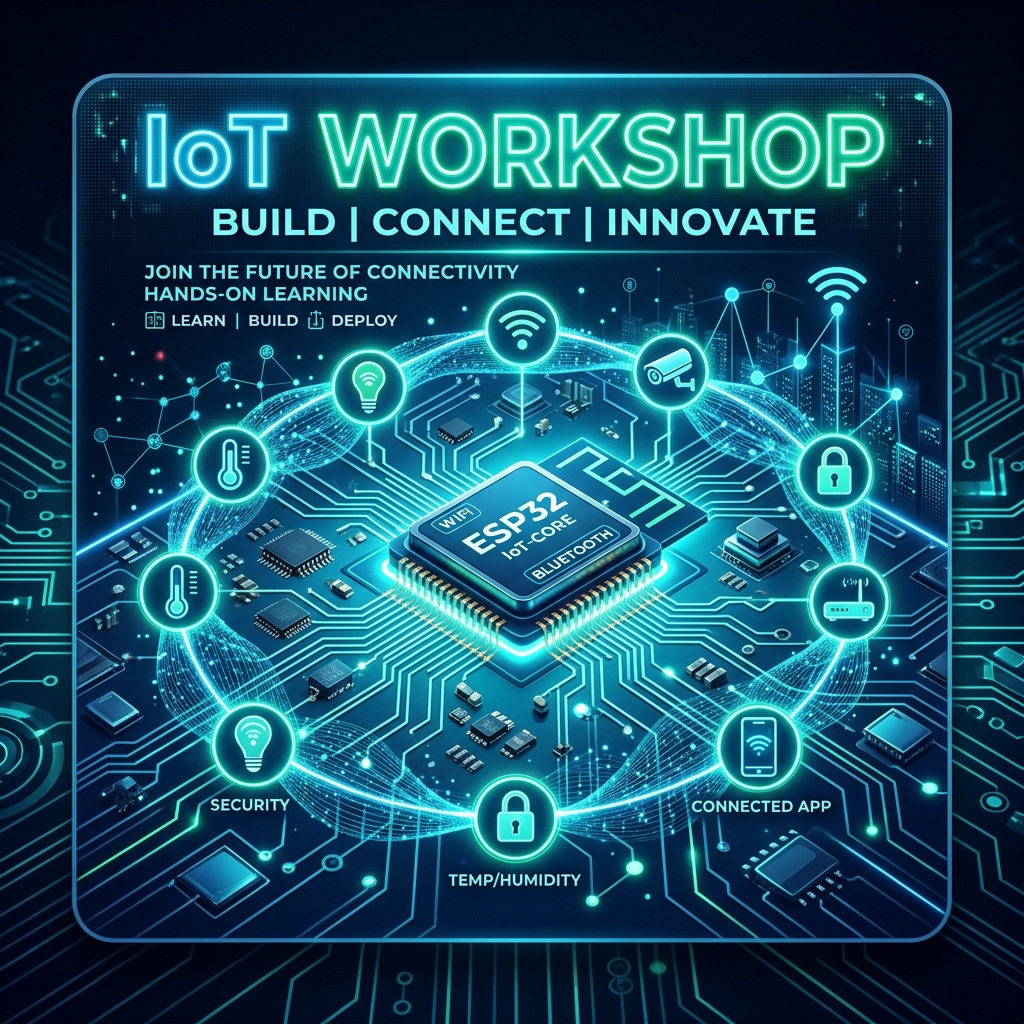
\includegraphics[width=\paperwidth]{iot_workshop_banner.png}};
    \end{tikzpicture}
\end{frame}
}

% --- Table of Contents ---
\begin{frame}{Agenda}
    \tableofcontents
\end{frame}

\section{What is IoT?}
\begin{frame}{What is the Internet of Things (IoT)?}
    \begin{itemize}
        \item \textbf{Definition}: A network of physical objects---``things''---that are embedded with sensors, software, and other technologies for the purpose of connecting and exchanging data with other devices and systems over the internet.
        \item \textbf{Evolution}:
            \begin{itemize}
                \item Pre-IoT: Isolated devices.
                \item Today: Ubiquitous connectivity (Smart homes, Industrial IoT, Healthcare).
            \end{itemize}
        \item \textbf{The Core Idea}: Making inanimate objects ``smart'' and ``connected''.
    \end{itemize}
\end{frame}

\section{The Brains of IoT}
\begin{frame}{Microcontroller (MCU) vs. Microprocessor (MPU)}
    \begin{columns}
        \column{0.5\textwidth}
        \textbf{Microcontroller (MCU)}
        \begin{itemize}
            \item All-in-one chip (CPU, RAM, Storage).
            \item Low power consumption.
            \item Designed for specific tasks.
            \item \textit{Examples}: ESP8266, ESP32, Arduino.
        \end{itemize}
        
        \column{0.5\textwidth}
        \textbf{Microprocessor (MPU)}
        \begin{itemize}
            \item CPU only (needs external RAM/Storage).
            \item High power, high speed.
            \item General-purpose computing.
            \item \textit{Examples}: Raspberry Pi, Intel i7, Apple M2.
        \end{itemize}
    \end{columns}
\end{frame}

\section{Introduction to NodeMCU}
\begin{frame}{Why NodeMCU?}
    \begin{itemize}
        \item \textbf{Low Cost}: Highly affordable for projects.
        \item \textbf{WiFi Integrated}: No extra modules needed for connectivity.
        \item \textbf{Open Source}: Large community support.
        \item \textbf{Arduino Compatible}: Easy to program using C/C++ syntax.
    \end{itemize}
    \centering
    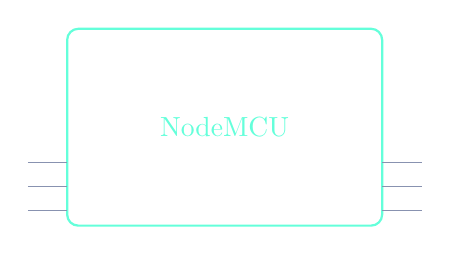
\begin{tikzpicture}
        \draw[IoTCyan, thick, rounded corners] (0,0) rectangle (4,2.5);
        \node at (2,1.25) {\textcolor{IoTCyan}{NodeMCU}};
        \draw[IoTGrey, ultra thin] (-0.5, 0.2) -- (0, 0.2);
        \draw[IoTGrey, ultra thin] (-0.5, 0.5) -- (0, 0.5);
        \draw[IoTGrey, ultra thin] (-0.5, 0.8) -- (0, 0.8);
        \draw[IoTGrey, ultra thin] (4, 0.2) -- (4.5, 0.2);
        \draw[IoTGrey, ultra thin] (4, 0.5) -- (4.5, 0.5);
        \draw[IoTGrey, ultra thin] (4, 0.8) -- (4.5, 0.8);
    \end{tikzpicture}
\end{frame}

\section{Sensors \& Actuators}
\begin{frame}{Physical Interface: Sensors \& Actuators}
    \begin{itemize}
        \item \textbf{Sensors (Input)}: 
            \begin{itemize}
                \item Eyes and ears of the system.
                \item Examples: LDR (Light), DHT11 (Temp/Humidity), Ultrasonic.
            \end{itemize}
        \item \textbf{Actuators (Output)}: 
            \begin{itemize}
                \item Hands and voice of the system.
                \item Examples: LEDs, Buzzers, Relays, Motors.
            \end{itemize}
    \end{itemize}
\end{frame}

\begin{frame}{Ready to Build?}
    \centering
    \Huge \textcolor{IoTCyan}{Let's get started!}
    
    \vspace{1cm}
    \large \textcolor{IoTGrey}{Next Session: Interfacing and Logic}
\end{frame}

\end{document}
